\documentclass[11pt,a4paper]{article}

\usepackage[utf8]{inputenc}
\usepackage[T1]{fontenc}
\usepackage[spanish]{babel}

\usepackage{tgpagella}
\usepackage{geometry}
\usepackage{booktabs}
\usepackage{xcolor}
\usepackage{graphicx}
\usepackage{titlesec}
\usepackage{fancyhdr}
\usepackage[parfill]{parskip}
\usepackage[expansion=false]{microtype}
\usepackage{hyperref}
\usepackage{setspace}
\usepackage{needspace}
\usepackage{etoolbox}
\usepackage{ragged2e}

\widowpenalty=10000
\clubpenalty=10000
\displaywidowpenalty=10000

\hyphenpenalty=8000
\exhyphenpenalty=8000

\geometry{top=3.0cm,bottom=3.0cm,left=3.5cm,right=3.5cm}

\setlength{\parskip}{0.65em}
\setlength{\parindent}{0em}

\definecolor{azulai}{RGB}{30,80,140}
\definecolor{doradoai}{RGB}{140,90,0}
\definecolor{grisai}{RGB}{70,70,70}

\AtBeginDocument{\justifying}

\titleformat{\section}
{\Large\bfseries\color{azulai}\justifying}
{}
{0em}
{}
[{\color{azulai}\titlerule[0.5pt]}]

\titlespacing*{\section}
{0pt}{1.3em}{0.5em}

\titleformat{\subsection}
{\large\bfseries\color{doradoai}\justifying}
{}
{0em}
{}

\titlespacing*{\subsection}
{0pt}{1.0em}{0.35em}

\titleformat{\subsubsection}
{\normalsize\bfseries\color{grisai}\justifying}
{}
{0em}
{}

\titlespacing*{\subsubsection}
{0pt}{0.8em}{0.25em}

\preto\section{\Needspace{8\baselineskip}}
\preto\subsection{\Needspace{6\baselineskip}}
\preto\subsubsection{\Needspace{4\baselineskip}}

\pagestyle{fancy}
\fancyhf{}

\rhead{\textcolor{grisai}{\small Maite Barragan — Arquitectura Interna}}
\lhead{\textcolor{grisai}{\small Mercurio · Venus · Marte}}
\cfoot{\textcolor{grisai}{\small\thepage}}

\renewcommand{\headrulewidth}{0.3pt}

\hypersetup{
colorlinks=true,
linkcolor=azulai,
urlcolor=azulai
}

\setstretch{1.32}

\tolerance=1500
\emergencystretch=4em

\begin{document}

% ── Portada ──────────────────────────────────────────────────────────────────

\begin{titlepage}
  \centering

  \vspace*{2cm}

  {\Huge\bfseries\color{azulai} Mercurio · Venus · Marte}\\[0.6cm]

  {\large\color{grisai} Arquitectura Interna}\\[0.4cm]

  {\small\itshape\color{grisai}
  Procesamiento, vínculo y acción en el funcionamiento cotidiano
  }\\[2.2cm]

  {\huge\color{doradoai} Maite Barragan}\\[1.6cm]

  {\Large 07/01/1971 \quad 12:15}\\[0.35cm]

  {\Large Pamplona, España}\\[0.35cm]

  {\normalsize
  Lat: 42.8157° \quad
  Lon: -1.6522° \quad
  UTC+01:00
  }\\[0.35cm]

  {\normalsize
  Ascendente: Aries 6°18'
  \quad
  MC: Capricornio 3°11'
  }\\[2.2cm]

  \renewcommand{\arraystretch}{1.35}

  \begin{tabular}{ll}
    \textbf{Mercurio:} & Sagitario — Casa 9 27°51' (Rx) \\
    \textbf{Venus:}    & Sagitario — Casa 8 0°23' \\
    \textbf{Marte:}    & Escorpio — Casa 8 20°09' \\
  \end{tabular}

  \vfill

  {\small\color{grisai}
  Generado el 20/05/2026
  }

\end{titlepage}

\justifying

\tableofcontents

\clearpage

% ── Datos de referencia ───────────────────────────────────────────────────────
\section{Datos de referencia}

\begin{center}
\renewcommand{\arraystretch}{1.25}
\begin{tabular}{llll}
  \toprule
  \textbf{Planeta} & \textbf{Signo} & \textbf{Casa} & \textbf{Posición} \\
  \midrule
  Mercurio (Rx)  & Sagitario  & 9  & 27°51' \\
  Venus    & Sagitario & 8 & 0°23' \\
  Marte    & Escorpio & 8 & 20°09' \\
  Ascendente          & Aries           & ---                    & 6°18' \\
  Medio Cielo         & Capricornio            & ---                    & 3°11' \\
  \bottomrule
\end{tabular}
\end{center}
\justifying

\vspace{0.5cm}

\textbf{Aspectos entre planetas personales:}

\vspace{0.3cm}\textit{No hay aspectos entre los planetas personales en los orbes definidos.}

\justifying

\vspace{0.7cm}

\begin{center}
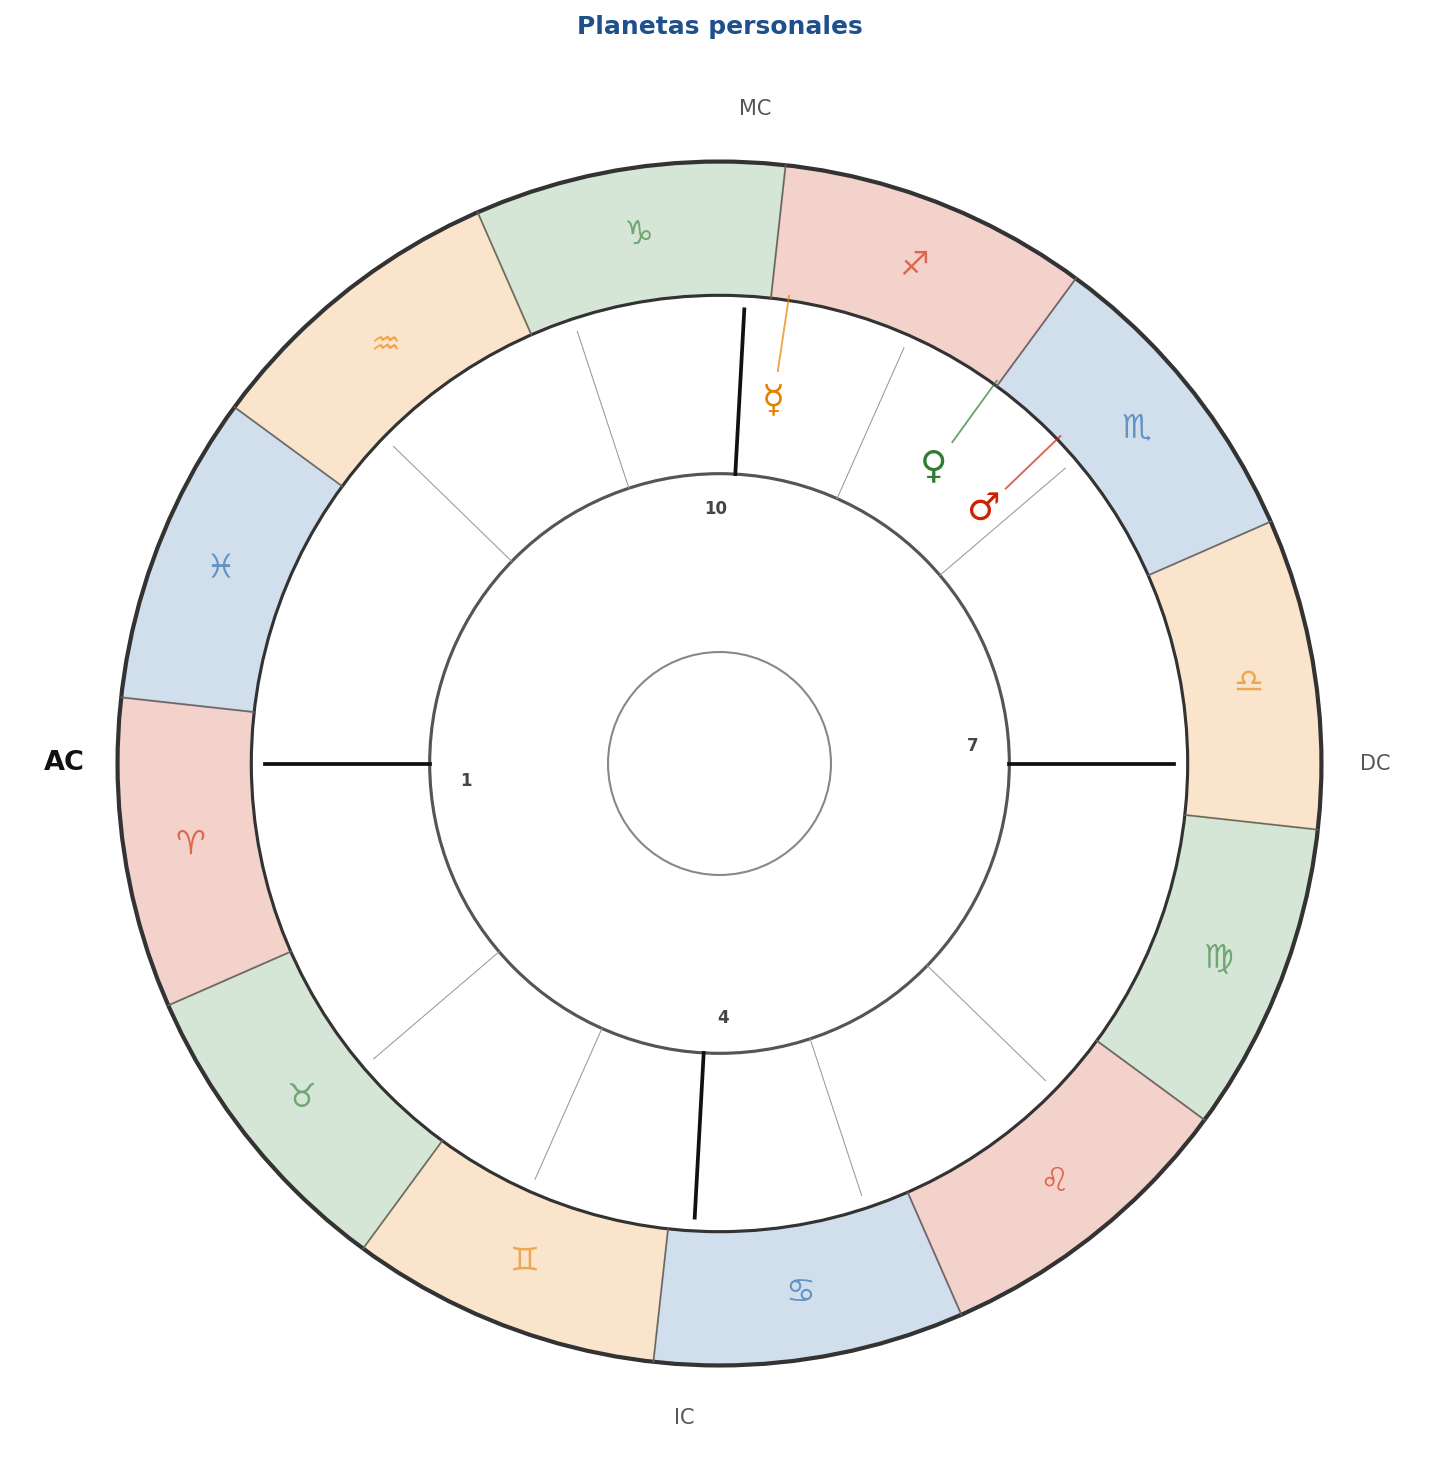
\includegraphics[width=0.72\textwidth]{Maite_Barragan_Planetas_Personales_rueda.png}
\end{center}

\vspace{0.3cm}
\Needspace{5\baselineskip}

% ── Interpretación ────────────────────────────────────────────────────────────
\section{Interpretación — Arquitectura Interna}

\begin{center}
{\small\itshape\color{grisai}
No se trata de describir la personalidad.\\
Se trata de observar cómo procesas, cómo te vinculas\\
y cómo se mueve tu energía en la vida cotidiana.
}
\end{center}

\justifying

\vspace{0.8cm}

% ── 1. Funcionamiento general ─────────────────────────────────────────────────
\subsection{1. Funcionamiento general}

\justifying
Mercurio está en Sagitario, Casa 9: muestra cómo piensas, cómo ordenas lo que percibes y cómo traduces lo que ocurre en palabras o ideas.
Venus está en Sagitario, Casa 8: muestra cómo te vinculas, qué necesitas para sentir conexión y cómo buscas equilibrio afectivo.
Marte está en Escorpio, Casa 8: muestra cómo se activa tu acción, cómo descargas energía y cómo respondes ante el impulso.

Hay una concentración funcional entre Venus, Marte. Estas dos áreas tienden a activarse de forma cercana. Cuando una se mueve, la otra suele implicarse también. Esto puede dar fluidez, pero también puede hacer que cueste separarlas bajo presión.

Hay coherencia elemental entre: tu forma de pensar (Mercurio) y tu forma de vincularte (Venus) comparten elemento: Fuego. Esto facilita que esas áreas colaboren entre sí. Aun así, lo que fluye con facilidad también puede volverse automático si no lo observas con consciencia.

Hay tensión elemental entre: tu forma de pensar (Mercurio, Fuego) y tu forma de actuar (Marte, Agua); tu forma de vincularte (Venus, Fuego) y tu forma de actuar (Marte, Agua). Esto no es un problema en sí mismo, pero sí pide más atención. Cuando esas áreas necesitan cooperar, conviene hacer una integración consciente para que una no bloquee, desborde o desconecte a la otra.

No aparecen aspectos clásicos entre los planetas personales dentro de los orbes definidos. Aun así, puede existir una concentración funcional si los planetas están próximos por signo, por casa o por continuidad de experiencia.

\vspace{0.8cm}

% ── 2. Mercurio ───────────────────────────────────────────────────────────────
\subsection{2. Mercurio — Pensamiento y procesamiento}

\subsubsection*{Mercurio en Sagitario — Casa 9 (Rx)}

\justifying
Tu mente funciona buscando sentido general y visión amplia. Necesitas comprender el marco mayor antes de entrar en los detalles. Cuando algo tiene dirección o propósito, la comprensión se vuelve mucho más fluida.

La saturación aparece cuando tienes que sostener detalle repetitivo durante demasiado tiempo sin acceso al conjunto completo. Entonces pierdes interés o generalizas demasiado rápido. El bloqueo suele aparecer cuando una idea ya se ha convertido en verdad absoluta: puedes seguir razonando desde un marco que ya no encaja con la realidad actual.

Sueles regularte mejor cuando puedes alternar visión amplia y realidad concreta sin perder contacto con ninguna de las dos.

Necesitas visión amplia y sentido general para organizar la mente. Comprendes mejor cuando puedes relacionar la información con una idea mayor, una filosofía o una dirección clara.

La saturación aparece cuando hay exceso de detalle sin contexto o tareas repetitivas sin significado visible. Entonces la atención se dispersa o pierde motivación. Sueles regularte mejor cuando puedes alternar aprendizaje amplio con aplicaciones concretas que den sentido a lo que haces.

Mercurio está retrógrado. Tu forma de procesar tiende a ser más interna y necesita más revisión antes de salir hacia afuera. Las conclusiones pueden llegar después de varias vueltas internas, y comunicar con claridad puede requerir más tiempo.

\vspace{0.8cm}

% ── 3. Venus ──────────────────────────────────────────────────────────────────
\subsection{3. Venus — Vínculo y regulación relacional}

\subsubsection*{Venus en Sagitario — Casa 8}

\justifying
Necesitas libertad, crecimiento y sensación de expansión compartida dentro del vínculo. La relación suele fortalecerse cuando permite explorar, aprender y mantener espacios propios además de los compartidos.

La saturación aparece cuando la relación se vive como limitación, exceso de control o rutina demasiado cerrada. Entonces la energía afectiva empieza a alejarse incluso antes de que exista conflicto abierto. Cuando el vínculo deja de sostenerse, tiendes a tomar distancia rápidamente para recuperar amplitud y movimiento.

Sueles regularte mejor en relaciones donde existe honestidad, movimiento y suficiente libertad para seguir creciendo.

Necesitas profundidad emocional e intimidad real para que una relación se sienta significativa. La conexión suele vivirse con intensidad y necesidad de acceso genuino al otro. Las relaciones superficiales rara vez te resultan suficientes.

La saturación aparece cuando percibes secretos, distancia emocional o sensación de conexión parcial. Entonces puedes entrar en vigilancia emocional o necesidad de entender qué ocurre realmente debajo de la superficie. Sueles regularte mejor mediante honestidad emocional, intimidad y vínculos donde exista confianza profunda.

\vspace{0.8cm}

% ── 4. Marte ──────────────────────────────────────────────────────────────────
\subsection{4. Marte — Acción y descarga}

\subsubsection*{Marte en Escorpio — Casa 8}

\justifying
Tu energía se activa con intensidad y concentración. Respondes con mucha fuerza cuando percibes amenaza, desafío o necesidad de transformación profunda. La acción descarga mediante enfoque, confrontación o procesos de cambio radical.

La saturación aparece cuando la energía queda acumulada sin salida clara. Entonces puedes entrar en estados de control excesivo, obsesión o activación interna permanente. La tensión retenida durante mucho tiempo puede descargarse de forma muy intensa cuando finalmente encuentra salida.

Sueles regularte mejor mediante actividad intensa, profundidad emocional y espacios donde puedas actuar con honestidad y enfoque.

Necesitas profundidad e intensidad para sentirte plenamente activade. Tu energía descarga mejor en procesos transformadores, vínculos profundos o experiencias emocionalmente intensas.

La saturación aparece cuando la energía queda contenida durante demasiado tiempo o no encuentra espacios de descarga profunda. Entonces puede aparecer control excesivo, tensión interna constante o sensación de activación acumulada difícil de soltar. Sueles regularte mejor mediante intensidad consciente, honestidad emocional y procesos reales de transformación.

\vspace{0.8cm}

% ── 5. Integración ────────────────────────────────────────────────────────────
\subsection{5. Integración — Coherencias, fricciones y bucles}

\justifying
Hay una integración fuerte entre Venus, Marte. Estas áreas se activan de manera cercana y conviene observarlas juntas. A veces una de ellas expresa la tensión que en realidad empezó en la otra.

Mercurio y Venus comparten elemento en Fuego. Tu forma de pensar y tu forma de vincularte pueden comprenderse con relativa facilidad. Suele haber continuidad entre lo que percibes, lo que sientes y lo que necesitas expresar en relación.

Mercurio (Sagitario, Fuego) y Marte (Escorpio, Agua) operan en elementos que crean tensión. Tu modo de procesar y tu modo de actuar no se alimentan de forma directa. Puede haber mucho pensamiento sin movimiento, o acción antes de que exista claridad suficiente.

Venus (Sagitario, Fuego) y Marte (Escorpio, Agua) operan en elementos que crean tensión. Lo que necesitas para conectar y lo que necesitas para actuar no siempre se refuerzan. Cuando hay demanda simultánea de vínculo y acción, puedes tender a priorizar una cosa a expensas de la otra.

Cuando hay demasiada presión, puede aparecer una cadena reconocible: Mercurio en Sagitario acelera hacia conclusiones antes de que el análisis esté completo. Desde ahí, Venus en Sagitario se aleja del vínculo o usa la relación como escenario de descarga. Y Marte en Escorpio se disipa o actúa en dirección del entorno antes que desde el propio impulso. El ciclo se cierra cuando la energía acumulada vuelve a saturar el punto inicial.

\vspace{0.8cm}

% ── 6. Orientación práctica ───────────────────────────────────────────────────
\subsection{6. Orientación práctica}

\subsubsection*{Desde dónde empezar}

\justifying
Desde tu forma de pensar (Mercurio) en Sagitario, Casa 9. De las tres áreas, esta suele requerir menos energía para activarse. La entrada es activar el movimiento antes de intentar resolverlo todo mentalmente. Empezar por aquí puede abrir movimiento en el resto.

\subsubsection*{Qué sostener}

\justifying
Conviene sostener especialmente tu forma de actuar (Marte) en Escorpio: tiempo de integración, silencio emocional y límites sensibles. Bajo presión, esta área puede desorganizarse antes que las demás. Cuando se estabiliza, el resto de tu funcionamiento tiene más capacidad para reorganizarse.

\subsubsection*{Qué evitar}

\justifying
Evitar asumir que la ausencia de fricción visible significa que todo está bien. A veces los bucles no hacen ruido porque te has acostumbrado a funcionar así.

\vspace{0.6cm}

\justifying
Si no se sostiene: pensamiento, vínculo y acción empiezan a funcionar por separado. Lo que piensas no alimenta la acción, la acción no informa al vínculo y el vínculo no regula la energía disponible. El esfuerzo aumenta, la claridad disminuye y la saturación llega antes.

\vspace{1.2cm}

\begin{center}
{\small\itshape\color{grisai}
La astrología se utiliza aquí como lenguaje simbólico de observación,\\
no como una definición cerrada de quién eres.\\[0.2cm]
Este documento propone una lectura funcional y orientativa, no un diagnóstico.
}
\end{center}

\end{document}
